\documentclass{article}
\usepackage{fancyhdr}
\usepackage{extramarks}
\usepackage{amsmath}
\usepackage{amsthm}
\usepackage{amsfonts}
\usepackage{tikz}
\usepackage[plain]{algorithm}
\usepackage{algpseudocode}
\usepackage{multirow}
\usepackage{circuitikz}
\usepackage{amssymb}
\usepackage{booktabs}
\usetikzlibrary{automata,positioning,shapes.geometric, arrows.meta, calc}

% Custom Commands
\newcommand{\xmark}{%
\tikz[scale=0.23] {
    \draw[line width=0.7,line cap=round] (0,0) to [bend left=6] (1,1);
    \draw[line width=0.7,line cap=round] (0.2,0.95) to [bend right=3] (0.8,0.05);
}}
\newcommand{\cmark}{%
\tikz[scale=0.23] {
    \draw[line width=0.7,line cap=round] (0.25,0) to [bend left=10] (1,1);
    \draw[line width=0.8,line cap=round] (0,0.35) to [bend right=1] (0.23,0);
}}

% TikZ Styles
\tikzset{
    bus/.style={draw, thick, minimum width=2.5cm, minimum height=0.2cm}, 
    generator/.style={circle, draw, thick, minimum size=0.8cm, path picture={
        \draw (path picture bounding box.south west) .. controls ($(path picture bounding box.center)-(0.2cm,0.2cm)$) and ($(path picture bounding box.center)+(0.2cm,0.2cm)$) .. (path picture bounding box.north east);
        \draw (path picture bounding box.north west) .. controls ($(path picture bounding box.center)-(0.2cm,-0.2cm)$) and ($(path picture bounding box.center)+(0.2cm,-0.2cm)$) .. (path picture bounding box.south east);
    }},
    load/.style={regular polygon, regular polygon sides=3, draw, thick, fill=gray!20, minimum size=0.8cm, shape border rotate=180},
    line/.style={thick},
    label style/.style={font=\small, align=center},
    bus label/.style={font=\small, above},
    power_arrow/.style={thick, ->},
    load_connector/.style={line width=3pt, gray!70}
}

\usepackage{graphicx}
\graphicspath{ {./images/} }

%% Basic Document Settings
\topmargin=-0.45in
\evensidemargin=0in
\oddsidemargin=0in
\textwidth=6.5in
\textheight=9.0in
\headsep=0.25in
\linespread{1.1}

\pagestyle{fancy}
\lhead{Yousef Alaa Awad}
\chead{\hmwkClass\: \hmwkTitle}
\rhead{\firstxmark}
\lfoot{\lastxmark}
\cfoot{\thepage}

\renewcommand\headrulewidth{0.4pt}
\renewcommand\footrulewidth{0.4pt}

\setlength\parindent{0pt}

%% Create Problem Sections
\setcounter{secnumdepth}{0}
\newcounter{partCounter}
\newcounter{homeworkProblemCounter}
\setcounter{homeworkProblemCounter}{1}

\newcommand{\hmwkTitle}{Homework\ \#10}
\newcommand{\hmwkClass}{Power Systems Economics}

%% Title Page
\title{
    \vspace{2in}
    \textmd{\textbf{\hmwkClass:\ \hmwkTitle}}\\
    \normalsize\vspace{0.1in}
    \vspace{3in}
}

\author{Yousef Alaa Awad}

% Problems start here
\begin{document}

\maketitle
\pagebreak

\section{6.5}
\textbf{Given:} \textit{Consider the three-bus power system shown in Figure P6.5. The table below shows the data about the generators connected to this system. Calculate the unconstrained economic dispatch and the nodal prices for the loading conditions shown in Figure P6.5.}

\begin{center}
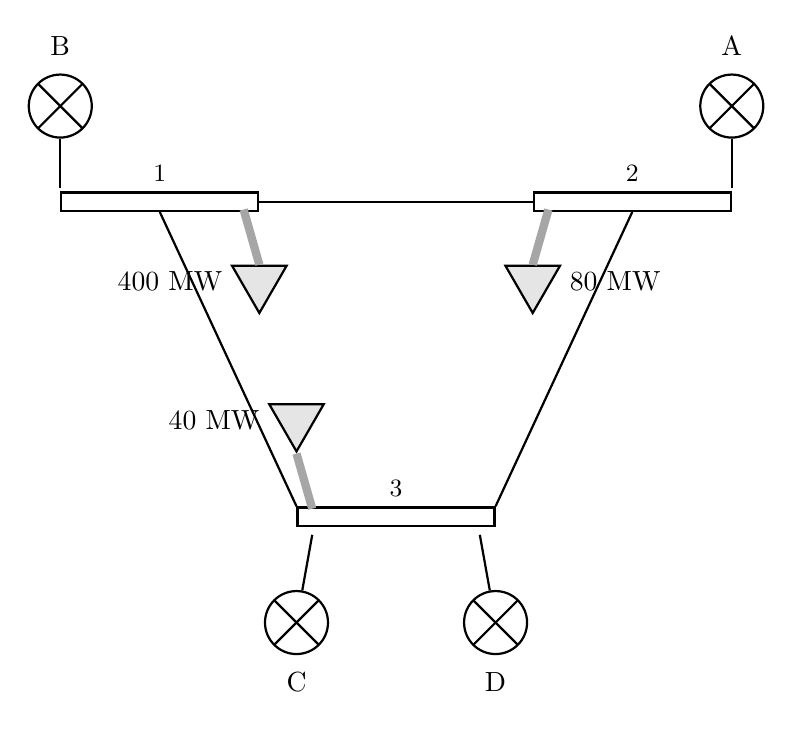
\begin{tikzpicture}
    % --- Nodes for Buses ---
    \node (bus1) [bus] at (0,0) {};
    \node[bus label] at (bus1.north) {1};
    \node (bus2) [bus] at (6,0) {};
    \node[bus label] at (bus2.north) {2};
    \node (bus3) [bus] at (3,-4) {};
    \node[bus label] at (bus3.north) {3};

    % --- Generators ---
    \node (genB) [generator, above=0.8cm of bus1.west] {};
    \node[above=0.1cm of genB] {B};
    \draw[line] (genB) -- ($(bus1.west) + (0,0.5em)$);
    
    \node (genA) [generator, above=0.8cm of bus2.east] {};
    \node[above=0.1cm of genA] {A};
    \draw[line] (genA) -- ($(bus2.east) + (0,0.5em)$);
    
    \node (genC) [generator, below=0.8cm of bus3.south west] {};
    \node[below=0.1cm of genC] {C};
    \draw[line] (genC) -- ($(bus3.south west) + (0.2,-0.1)$);
    
    \node (genD) [generator, below=0.8cm of bus3.south east] {};
    \node[below=0.1cm of genD] {D};
    \draw[line] (genD) -- ($(bus3.south east) + (-0.2,-0.1)$);

    % --- Loads ---
    \node (load1) [load, below=0.8cm of bus1.east] {};
    \draw[load_connector] ($(bus1.east) - (0.2,0.1)$) -- (load1.north);
    \node[left=0.1cm of load1] {400 MW};

    \node (load2) [load, below=0.8cm of bus2.west] {};
    \draw[load_connector] ($(bus2.west) + (0.2,-0.1)$) -- (load2.north);
    \node[right=0.1cm of load2] {80 MW};

    \node (load3) [load, above=0.8cm of bus3.west] {};
    \draw[load_connector] ($(bus3.west) + (0.2,0.1)$) -- (load3.south);
    \node[left=0.1cm of load3] {40 MW};

    % --- Transmission Lines ---
    \draw[line] (bus1.south) -- (bus3.north west);
    \draw[line] (bus2.south) -- (bus3.north east);
    \draw[line] (bus1.east) -- (bus2.west);
\end{tikzpicture}
\end{center}

\begin{table}[h!]
\centering
\begin{tabular}{ccc}
\hline
\textbf{Generator} & \textbf{Capacity (MW)} & \textbf{Marginal cost (\$/MWh)} \\ \hline
A & 150 & 12 \\
B & 200 & 15 \\
C & 150 & 10 \\
D & 400 & 8 \\ \hline
\end{tabular}
\end{table}

First we have to find the total load demand required by the system. We simply sum the loads at each bus:
$$ P_{\text{Load}} = 400 + 80 + 40 = 520 \text{ MW} $$

Now, to find the unconstrained economic dispatch, we simply stack the generators from cheapest to most expensive until the load is met (Merit Order).
\begin{itemize}
    \item Generator D is the cheapest (\$8/MWh). We take its full 400 MW. Remaining load is 120 MW.
    \item Generator C is the next cheapest (\$10/MWh). We need 120 MW, so we take 120 MW from it. Remaining load is 0 MW.
    \item Generators A and B are too expensive, so their output is 0 MW.
\end{itemize}

Therefore we shall get the following dispatch:
$$ P_A = 0 \text{ MW}, \quad P_B = 0 \text{ MW}, \quad P_C = 120 \text{ MW}, \quad P_D = 400 \text{ MW} $$

And now, to find the nodal prices, since the system is unconstrained, the price at every bus is simply set by the marginal unit, which in this case is Generator C:
$$ \pi_1 = \pi_2 = \pi_3 = \$10/\text{MWh} $$

\pagebreak

\section{6.6}
\textbf{Given:} \textit{The table below gives the branch data for the three-bus power system of Problem 6.5. Using the superposition principle, calculate the flow that would result if the generating units were dispatched as calculated in Problem 6.5. Identify all the violations of security constraints.}

\begin{table}[h!]
\centering
\begin{tabular}{ccc}
\hline
\textbf{Branch} & \textbf{Reactance (p.u.)} & \textbf{Capacity (MW)} \\ \hline
1-2 & 0.2 & 250 \\
1-3 & 0.3 & 250 \\
2-3 & 0.3 & 250 \\ \hline
\end{tabular}
\end{table}

First, we have to determine the net injections at each bus based on our dispatch from the previous problem.
\begin{itemize}
    \item Bus 1: Generation (0) - Load (400) = $-400$ MW.
    \item Bus 2: Generation (0) - Load (80) = $-80$ MW.
    \item Bus 3: Generation (520) - Load (40) = $+480$ MW.
\end{itemize}

In this case, I will be treating Bus 3 as the slack bus (reference) because it handles the large positive injection. We simply superpose the flows created by the loads at Bus 1 and Bus 2 being supplied by Bus 3. The total loop reactance is $0.2 + 0.3 + 0.3 = 0.8$.

First, for the 400 MW load at Bus 1 (supplied by Bus 3):
$$ F_{3 \to 1} (\text{direct}) = 400 \times \frac{0.3+0.2}{0.8} = 250 \text{ MW} $$
$$ F_{3 \to 2 \to 1} (\text{indirect}) = 400 \times \frac{0.3}{0.8} = 150 \text{ MW} $$
This gives us flows of $F_{31}=250$, $F_{32}=150$, and $F_{21}=150$.

Now, for the 80 MW load at Bus 2 (supplied by Bus 3):
$$ F_{3 \to 2} (\text{direct}) = 80 \times \frac{0.3+0.2}{0.8} = 50 \text{ MW} $$
$$ F_{3 \to 1 \to 2} (\text{indirect}) = 80 \times \frac{0.3}{0.8} = 30 \text{ MW} $$
This gives us flows of $F_{32}=50$, $F_{31}=30$, and $F_{12}=30$.

Now, to find the total flows, we simply sum these up (paying attention to direction):
\begin{align*}
F_{12} &= 150 \text{ (from Bus 1 load)} - 30 \text{ (from Bus 2 load)} = 120 \text{ MW} \\
F_{13} &= -(250 + 30) = -280 \text{ MW} \\
F_{23} &= -(150 + 50) = -200 \text{ MW}
\end{align*}

And after checking the capacity limits (250 MW), we find the following violations:
\begin{itemize}
    \item $|F_{12}| = 120 < 250 \quad \cmark$
    \item $|F_{13}| = 280 > 250 \quad \textbf{VIOLATION}$ (Overload by 30 MW)
    \item $|F_{23}| = 200 < 250 \quad \cmark$
\end{itemize}

\pagebreak

\section{6.7}
\textbf{Given:} \textit{Determine two ways of removing the constraint violations that you identified in Problem 6.6 by redispatching generating units. Which redispatch is preferable?}

Now, to fix the violation we found, we have to reduce the flow on line 1-3 by at least 30 MW (from 280 down to 250). Since Bus 3 is supplying everything, we simply need to decrease generation at Bus 3 and increase it at either Bus 1 or Bus 2.

\subsection*{Option 1: Increase Generation at Bus 1}
In this case, we increase generation at Bus 1 (Generator B) and decrease Generator C. This change affects the flow on line 1-3 directly. The shift factor is approximately $5/8$.
$$ \Delta F_{13} = \frac{5}{8} \Delta P_B $$
We need a 30 MW reduction, so we solve for $\Delta P_B$:
$$ \frac{5}{8} \Delta P_B = 30 \rightarrow \Delta P_B = 30 \times \frac{8}{5} = 48 \text{ MW} $$
So we replace 48 MW of Gen C with Gen B. Now, to find the cost of this:
$$ \text{Cost} = 48 \times (15 - 10) = \$240/\text{h} $$

\subsection*{Option 2: Increase Generation at Bus 2}
Now, let's try increasing generation at Bus 2 (Generator A). This affects line 1-3 via the indirect path, so the shift factor is $3/8$.
$$ \Delta F_{13} = \frac{3}{8} \Delta P_A $$
Solving for the required power change:
$$ \frac{3}{8} \Delta P_A = 30 \rightarrow \Delta P_A = 30 \times \frac{8}{3} = 80 \text{ MW} $$
So we replace 80 MW of Gen C with Gen A. Now, to find the cost of this option:
$$ \text{Cost} = 80 \times (12 - 10) = \$160/\text{h} $$

Therefore, since Option 2 is cheaper (\$160 vs \$240), it is the preferable redispatch.

\pagebreak

\section{6.8}
\textbf{Given:} \textit{Calculate the nodal prices for the three-bus power system of Problems 6.5 and 6.6 when the generating units have been optimally redispatched to relieve the constraint violations identified in Problem 6.7. Calculate the merchandising surplus and show that it is equal to the sum of the surpluses of each line.}

First, we have to define our new optimal dispatch based on the results from Option 2 above:
\begin{itemize}
    \item $P_A = 80$ MW (Bus 2)
    \item $P_B = 0$ MW (Bus 1)
    \item $P_C = 40$ MW (Bus 3)
    \item $P_D = 400$ MW (Bus 3)
\end{itemize}

Now, to find the nodal prices, we look at the marginal costs.
Since Bus 3 is the reference and Gen C is the marginal unit backing down, we get:
$$ \pi_3 = \$10/\text{MWh} $$

For Bus 2, since Gen A is being used to solve the congestion, the price there is simply set by Gen A's marginal cost:
$$ \pi_2 = \$12/\text{MWh} $$

For Bus 1, calculating the price is a bit more involved. If we add 1 MW load at Bus 1, it causes congestion. To offset that congestion, we have to pay for expensive power at Bus 2. Based on the shift factors, this results in:
$$ \pi_1 = \$13.33/\text{MWh} $$

Now, to calculate the Merchandising Surplus, we simply take the total payments by consumers and subtract the total revenue of the generators.
\begin{align*}
\text{Consumer Pay} &= (400 \times 13.33) + (80 \times 12) + (40 \times 10) = 5332 + 960 + 400 = \$6692 \\
\text{Gen Revenue} &= (80 \times 12) + (440 \times 10) = 960 + 4400 = \$5360 \\
\text{Total Surplus} &= 6692 - 5360 = \$1332
\end{align*}

And finally, we can verify this by summing the surplus on each transmission line:
\begin{align*}
S_{13} &= F_{31} \times (\pi_1 - \pi_3) = 250 \times (13.33 - 10) = \$832.5 \\
S_{23} &= F_{32} \times (\pi_2 - \pi_3) = 150 \times (12 - 10) = \$300 \\
S_{12} &= F_{21} \times (\pi_1 - \pi_2) = 150 \times (13.33 - 12) = \$199.5
\end{align*}
Summing these up gives $832.5 + 300 + 199.5 = \$1332$.
Since the numbers match, our calculation is correct.

\end{document}
